\section{Case Study Settings}
The goal of this study is to evaluate the behavior of the WRF mesoscale model in its LES mode when forced up to 3m mesh size and incorporating surface data assimilation to solve the structures developed within the PBL. Five experiments were developed for this purpose. The first two were carried out at Høvsøre for the case without (H2) and with (H2) data assimilation. The last three correspond to simulations made in the Bolund Hill for the case without (B1) and with (B2-B3) data assimilation. Case B3 corresponds to a simulation with data assimilation of extrapolated surface values.

%El objetivo de este estudio es evaluar el comportamiento del modelo mesoescala WRF en su modo LES al ser exigido hasta tamaños de malla de 5m incorporando asimilación de datos superficiales para resolver las estructuras que se desarrollan dentro de la CLP. Para esto se desarrollaron 5 experimentos. Los primeros dos se llevaron a cabo en Høvsøre para el caso con (H1) y sin (H2) asimilación de datos. Los últimos tres corresponden a simulaciones hechas en la colina de Bolund para el caso sin (B1) y con (B2-B3) asimilación de datos. El caso B3 corresponde a una simulación con asimilación de datos de valores extrapolados de la superficie.

\subsection{Høvsøre Setup (H1 and H2)}
Høvsøre is a wind turbine test site located in Denmark. Historically, many studies have been conducted at this site because of its relatively homogeneous and flat surface \citep{Pea2015, Pea2013}, and therefore it is useful to validate numerical results of experimental models. The site counts with a meteorological mast, whose data are public, facilitating the access to the measurements for the data assimilation process \citep{floors2013wind}.

The simulation performed consists of a total of 14 hours, where the first 6 correspond to the spinup of the model and the time window where the data assimilation is applied. The date of the simulation were selected in such a way that it corresponds to a period with neutral atmospheric stability as declared by \cite{Pea2013} in its case 5. Table \ref{tab:05_config_hov} shows the main aspects of the H1 and H2 experiments.
%La simulación realizada consta en total de 14 horas, en donde las primeras 6 corresponden al spinup del modelo y a la ventana de tiempo en donde se aplicará la asimilación de datos. El día y la fecha de simulación se seleccionaron de tal manera que corresponde a un periodo con estabilidad atmosférica neutra según lo declarado por \cite{Pea2013} en su caso 5. La Tabla \ref{tab:05_config_hov} muestra los aspectos generales de los experimentos H1 y H2.

\begin{table}[h!]
	\caption{Numerical domain for H1 and H2 experiments.}\label{tab:05_config_hov}
	\centering
	\begin{tabular}{lr}
		\toprule
		Parameter & Selection \\
		\midrule
		Date	 	 & 2010-09-08 06:00:00  to 20:00:00 UTC  \\
		%Start	 	 & 06:00:00   UTC \\
		%End 		 & 20:00:00 UTC  \\
		%Nodes	 	 & $107\times107\times37$   \\
		Top BC	& 30000 [Pa]\\
		\# Domains	& 7   \\
		Domain Centre	& (56.440588, 8.150896)   \\
		%Lon. Centro	& 8.150896   \\
		%Interválo Salida & 10 [min]\\
		%Nodes & 2.831.472\\
		\bottomrule
	\end{tabular}
\end{table}

The initial condition and the boundary condition for the coarser mesh is given by the operational analysis of the GFS global model with 0.5$^\circ$ of resolution. The boundary condition is mapped to the first domain contours using a buffer zone of 5 elements of mesh and are updated every 6 hours. 

The extension configuration of the domains was subjected to a sensitivity analysis in order to adjust the best values in order to ensure: (i) the model stability, (ii) the convergence of results for the boundary layer and (iii) the lowest computation time. In this fashion, the number of elements for the mesh and the top boundary condition are established. The number of nodes in all the domains are set as $107\times107\times37$.

\begin{table}
	\caption{Characteristic values and databases of each domain for H1 and H2.}\label{tab:05_caract_hov}
	\centering
	\begin{tabular}{lrrrrrrr}
		\toprule
		Domain 				& d1	&	d2	&	d3	&	d4	&	d5	&	d6 &	d7 \\
		\midrule
		%$N_x$		& 107 & 107 & 107 &107&107&107&107  \\
		%$N_y$	 		& 107 & 107 & 107 &107&107&107&107  \\
		$\Delta x=\Delta y$	[m]	 		& 30000 & 10000 & 3333.3 &1111.1&222.22&74.074&24.691  \\
		$\Delta t$	[s]	 		& 75 & 25 & 8.333 &2.778&0.556&0.185&0.062  \\
		Terrain DB		 	& GMTED & GMTED & GMTED &ASTER&ASTER&ASTER&ASTER  \\
		LU DB					& USGS & USGS & USGS &CLC12&CLC12&CLC12&CLC12 \\
		\bottomrule
	\end{tabular}
\end{table}
For the downscaling, 7 nested domains with feedback were used, all of which were centered on the meteorological mast location. The subdomains were selected to avoid the double weighting due to the turbulent grey zone using a ratio of 5 for the telescopic generation of the d4 and d5 domains, where the shift to the microscale occurs (a technique validated by \cite{Green2015}). A spatial reference of the nested domain distribution can be seen in Figure \ref{fig:05_dom_hov}.
%Para la reducción de escalas, se utilizaron 7 dominios anidados con feedback centrados en el punto del mástil meteorológico. La selección de subdominios se hizo de tal forma de evitar la doble ponderación debido a la zona gris de la turbulencia, esto se llevó a cabo utilizando una reducción con razón de 5 en la generación telescópica de los dominios d4 y d5 donde ocurre el paso a la microescala (técnica validada por \cite{Green2015} ). Una referencia satelital de la distribución de dominios anidados se puede ver en la Figura \ref{fig:05_dom_hov}.

The simulation's high resolution is achieved through the implementation of non-native WRF databases. The ASTER database is used for the terrain height. For land use, the Corine 2012 database transformed to its analogue USGS24 is used for the interpretation of the code \citep{Pineda2004}. A value of $z_0=1.5$ [cm] is manually assigned for the surface of the innermost domain \citep{Pea2013}. The Table \ref{tab:05_caract_hov} shows the differences of each subdomain.
%La alta resolución de la simulación es alcanzada a través de la implementación de bases de datos no nativas del WRF. Para la altura del terreno se utiliza la base de datos ASTER. Para el uso de suelo se utiliza la base de datos Corine del 2012 transformada a su análogo USGS24 para la interpretación del código \citep{Pineda2004}. Manualmente se asigna un valor de $z_0=1.5$ [cm] para el suelo del dominio mas interior \citep{Pea2013}. La Tabla \ref{tab:05_caract_hov} muestra las diferencias de cada subdominio.

\begin{figure}
	\centering
	\begin{minipage}{0.5\linewidth}
		\center \hspace{2.8cm}(a)
	\end{minipage}%
	\begin{minipage}{0.5\linewidth}
		\center\hspace{-2.8cm}(b)
	\end{minipage}%
	
	\includegraphics[width=0.3\linewidth,trim={0cm 0cm -0cm 0cm},clip,frame]{Imagenes/05/hov_dom1_edit.jpg}\hspace{0.5cm}%
	\includegraphics[width=0.3\linewidth,trim={0cm 0cm 0cm 0cm},clip,frame]{Imagenes/05/hov_dom2_edit.jpg}\vspace{0.3cm}%
	
	\begin{minipage}{0.5\linewidth}
		\center \hspace{2.4cm}(c)
	\end{minipage}%
	\begin{minipage}{0.5\linewidth}
		\center \hspace{-2.8cm}(d)
	\end{minipage}%

	\includegraphics[width=0.3\linewidth,trim={2.5cm 6.5cm 2cm 3.5cm},clip]{Imagenes/05/hov_control_point.pdf}%
	\includegraphics[width=0.4\linewidth,trim={0.5cm 4cm 0cm 3cm},clip]{Imagenes/05/mesh57}%
	
	\caption{Simulation domains for H1 and H2. (a) Domains d1-d4. (b) d5-d7. (c) Detail of d7 with the control point. (d)  Vertical grid distribution on a 4:1 scale.}
	\label{fig:05_dom_hov}
\end{figure}

For the vertical mesh, special care is taken to refine it so it is consistent with the application of the LES. In the first level there is an aspect ratio of $\Delta_x/\Delta_{z_1}=2.35$ and this is progressively reduced in the higher levels. Figure \ref{fig:05_dom_hov}(d) shows the mesh detail for the first 500m in the vertical.
%Para la malla vertical se tiene especial cuidado de refinar de tal manera que sea consistente con la aplicación del LES. En el primer nivel se tiene una relación de aspecto de $\Delta_x/\Delta_{z_1}=2.35$ y esta va disminuyendo progresivamente en los niveles superiores. La Figura \ref{fig:05_dom_hov}(d) muestra el detalle de la malla para los primeros 500m en la vertical.

The selection of the settings was made in agreement with other similar works in the literature and can be seen in Table \ref{tab:05_param_hov}.
%La selección de las parametrizaciones se realizó en concordancia con otros trabajos parecidos en la literatura y se pueden ver en la Tabla \ref{tab:05_param_hov}.
\begin{table}
	\caption{Model physics for H1 and H2.}\label{tab:05_param_hov}
	\centering
	\begin{tabular}{lrrrrrrr}
		\toprule
		Domain 				& d01	&	d02	&	d03	&	d04	&	d05	&	d06 &	d07 \\
		\midrule
		Micro-physics		 	& WSM5 & WSM5 & WSM5 &WSM5&WSM5&WSM5&WSM5  \\
		Cumulus			 		& Grell & Grell & -- & -- & -- & -- & -- \\ 
		Superficial Layer	& MYNN & MYNN & MYNN & MYNN & MYNN & MYNN & MYNN \\
		PBL				 		& MYNN & MYNN & MYNN & MYNN & -- & -- & -- \\
		LES model				 		& -- & -- & -- & -- & 1.5TKE & 1.5TKE & 1.5TKE \\
		$c_k$				 		& -- & -- & -- & -- & 0.3 & 0.3 & 0.3 \\
		Soil model 		& Difus. & Difus. & Difus. & Difus. & Difus. & Difus. & Difus. \\
		LWR & RRTM &RRTM&RRTM&RRTM&RRTM&RRTM&RRTM \\
		SWR	& Dudhia &Dudhia&Dudhia&Dudhia&Dudhia&Dudhia&Dudhia \\
		\bottomrule
	\end{tabular}
\end{table}

Finally, the public data from the meteorological mast were used to feed the data assimilation process. The frequency at which the background is corrected is set at 10 minutes and is performed during the first 6 hours of the simulation. The variables that were assimilated are wind speed and direction, and are assimilated at 5 heights: 10, 40, 60, 80 and 100 meters above the ground.
%Finalmente, se utilizaron los datos públicos del mástil meteorológico para alimentar el proceso de asimilación de datos. La frecuencia con la cual se corrige el background es de 10 minutos y se realiza durante las primeras 6 horas de simulación. La variables variables asimiladas son la rapidez y dirección del viento, y se asimilan en 5 alturas: 10, 40, 60, 80 y 100 metros sobre el suelo.





%%BOLUND%%
\subsection{Bolund Setup (B1, B2 and B3)}
Bolund is a 12 [m] high, 130 [m] long and 75 [m] wide seaside hill located in Denmark. Thanks to the measurement campaign made by \cite{Bechmann2009}  and its posterior blind model comparison \citep{Berg2011,Bechmann2011}, this is an optimal location for the testing of experimental computational models in the context of complex terrain. The measurement campaign provides Bolund with information on 10 masts distributed across and close to the hill, as well as high resolution data for terrain height and roughness length.

%Bolund es una colina costera de 12 [m] de alto, 130 [m] de largo y 75 [m] de ancho ubicada en Dinamarca. Debido a la campaña de medición hecha por \cite{Bechmann2009} y a su posterior comparación ciega de modelos \citep{Berg2011,Bechmann2011} este es un lugar ideal para la prueba de modelos experimentales. La campaña de medición dota a bolund con información en 10 mástiles distribuidos sobre y en las cercanías de la colina, además de datos en alta resolución para la altura del terreno y el largo de rugosidad.

The conducted experiments consisted of 9 hours of simulation, with the first 6 hours being the spinup of the model. The date was selected according to what was declared by  \cite{Bechmann2009} for a day with the most neutral stratification possible. More information is presented in the Table \ref{tab:05_config_bol}.
%Los experimentos realizados consisten en 9 horas de simulación, siendo las primeras 6 el spinup del modelo. La fecha se seleccionó acorde a lo declarado por \cite{Bechmann2009} para un día con estratificación lo mas neutra que se pueda. Más información se presenta en la Tabla \ref{tab:05_config_bol}.

\begin{table}[h!]
	\caption{Numerical domain for B1, B2 and B3 experiments.}\label{tab:05_config_bol}
	\centering
	\begin{tabular}{lrr}
		\toprule
		Parameter & Selection \\
		\midrule
		Date	 	 & 29-12-2007 06:00 to 15:00 UTC \\
		%Hora Inicio	 	 & 06:00 UTM\\
		%Hora Término	 		 & 15:00 UTM\\
		$N_z$	 	 & 41   \\
		Top BC	& 30000 [Pa]\\
		\# Domains	& 8   \\
		Domain Centre	& (55.703474, 12.098854)   \\
		Nodes & 3.465.000\\
		\bottomrule
	\end{tabular}
\end{table}

De la misma forma que para el caso de Høvsøre, las condiciones iniciales y de borde proveninen del modelo GFS. Debido a las dimensiones de la colina, se utilizaron 8 dominios anidados para el escalamiento dinámico como se puede ver en la Figura \ref{fig:05_dom_bol}. Todos los dominios constan de $107\times107$ nodos en la horizontal, exeptuando el dominio mas interior d8 que es de $107\times92$ debido a la extensión de la base de datos entregada por la campaña de medición. Para el manejo de la zona gris se utiliza el mismo acercamiento que para los experimentos H1 y H2.

\begin{figure}[H]
	\begin{minipage}{0.05\linewidth}
		\hfill
	\end{minipage}%
	\begin{minipage}{0.3\linewidth}
		\center \hspace{-3mm}(a)
	\end{minipage}%
	\begin{minipage}{0.3\linewidth}
		\center (b)
	\end{minipage}%
\begin{minipage}{0.3\linewidth}
	\center (c)
\end{minipage}%
\begin{minipage}{0.05\linewidth}
\end{minipage}%

	\centering
	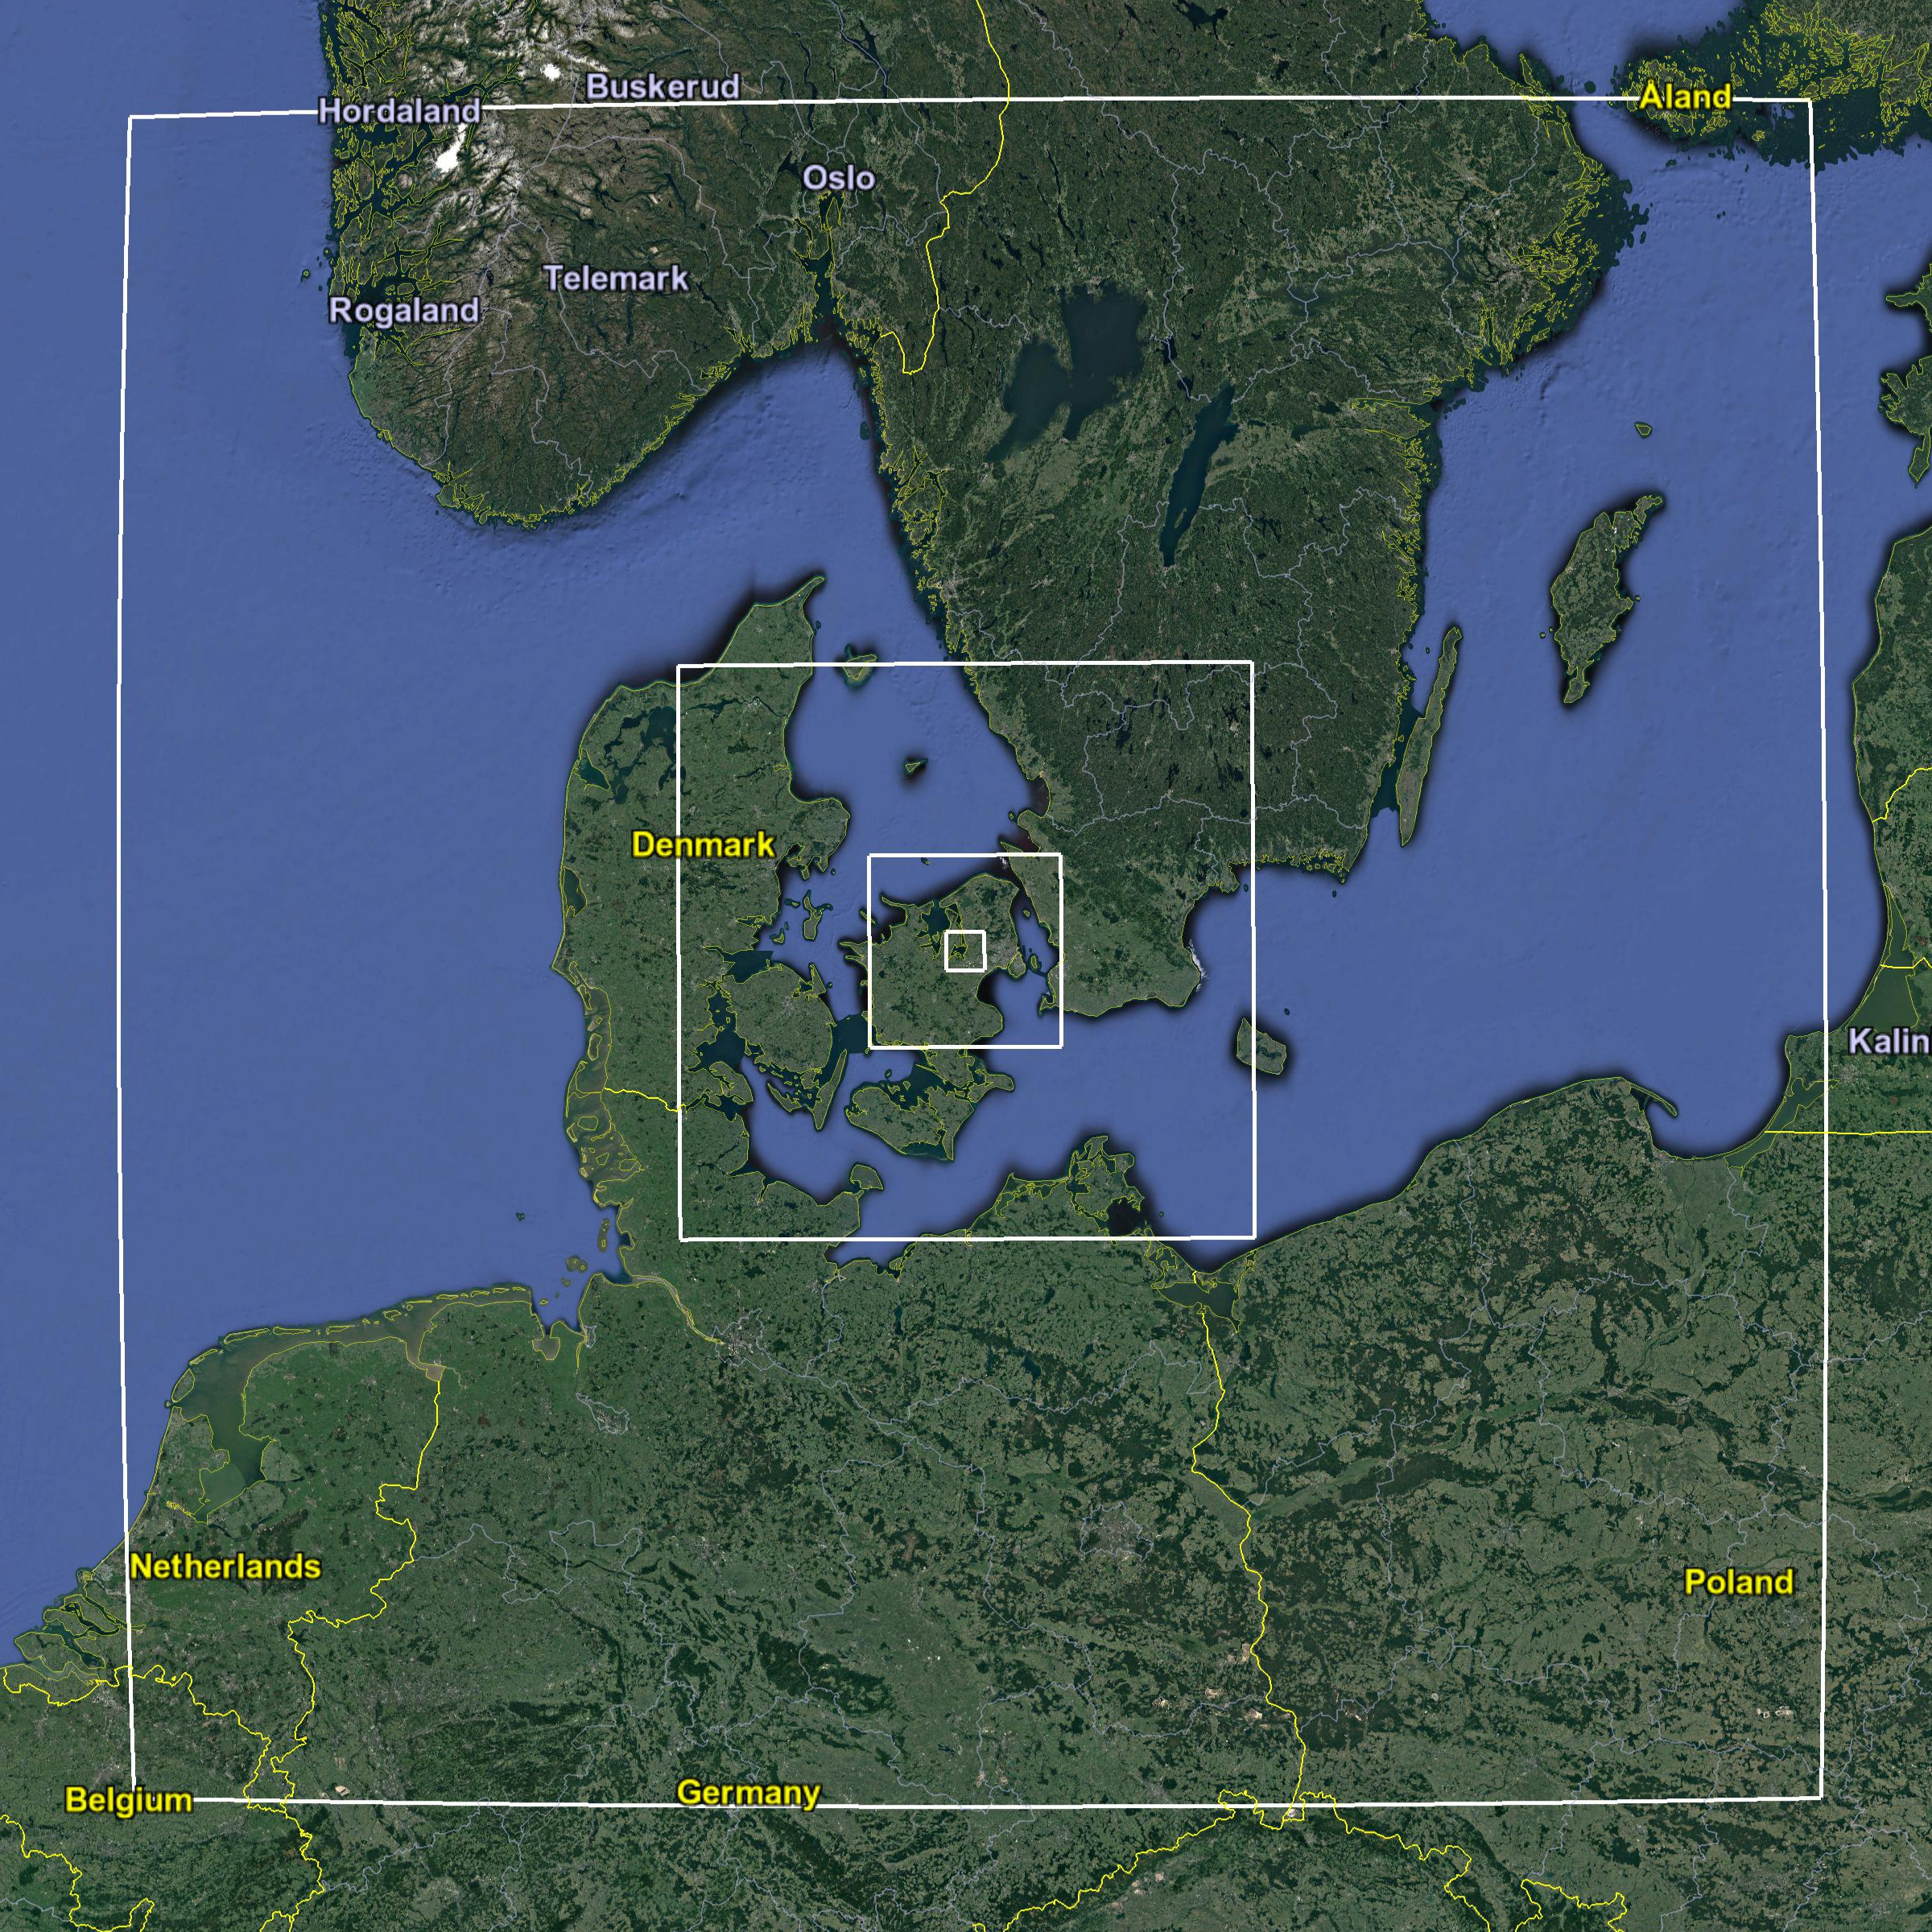
\includegraphics[width=0.3\linewidth,page=1,trim={5mm 3mm 3mm 3mm},clip,frame]{Imagenes/05/bol_d1-2-3-4edit.jpg}
	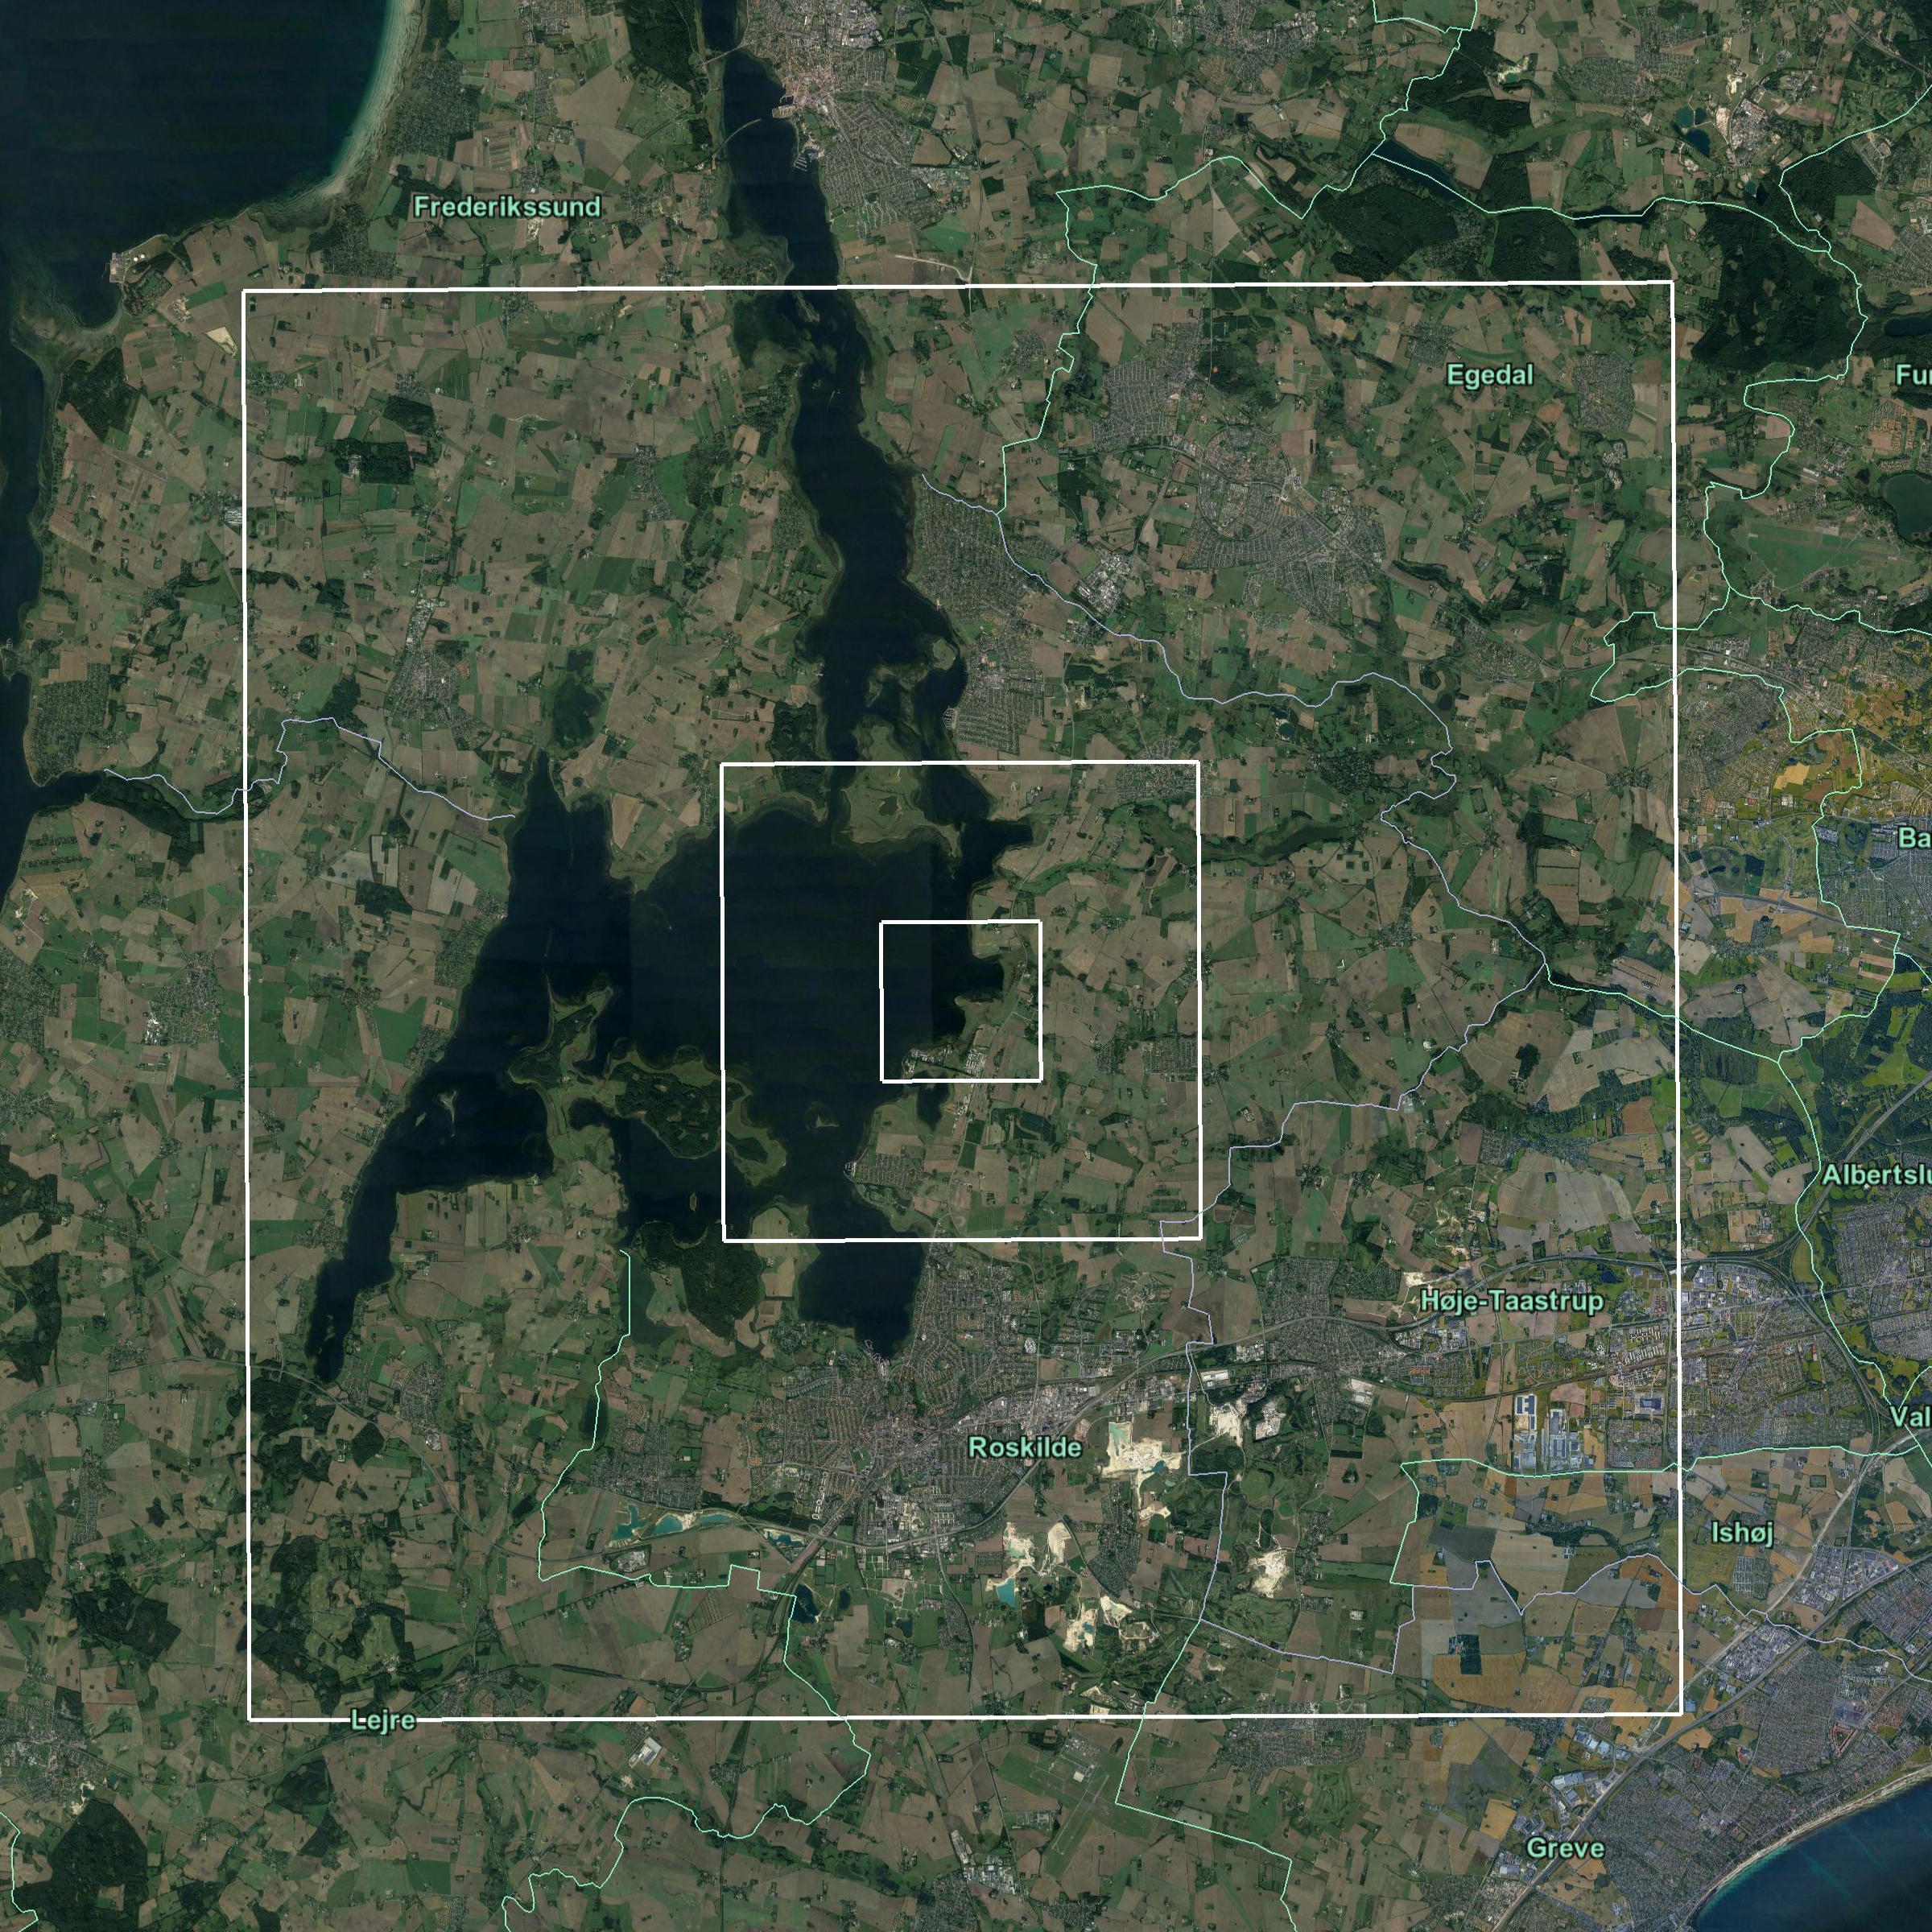
\includegraphics[width=0.3\linewidth,page=1,trim={5mm 3mm 3mm 3mm},clip,frame]{Imagenes/05/bol_d4-5-6edit.jpg}
	\includegraphics[width=0.3\linewidth,page=1,trim={5mm 3mm 3mm 3mm},clip,frame]{Imagenes/05/bol_d6-7-8edit.jpg}%
	
	\caption{Simulation domains for B1, B2 and B3. (a) d1-d4. (b) d4-d6. (c) d6-d8.}
	\label{fig:05_dom_bol}
\end{figure}

Con respecto a la alta resolución, se vuelven a utilizar las bases de datos CLC12 y ASTER para los dominios intermedios. Para el dominio d8 se incorporaron a WRF las bases de datos de uso de suelo y altura del terrono entregadas por los desarrolladores de la campaña de medición. Estas bases de datos poseen una resolución de 25 [cm], lo cual es suficiente para la malla mas interior con resolución de 3 [m]. El largo de rugosidad se fija en $z_0=1.5$ [cm] \citep{Bechmann2011}.

Debido a la pendiente abrupta de la colina, un refinamiento de la malla vertical fue realizado para evitar inestabilidades. De esta manera se fija la cantidad de nodos en la vertical como $N_z=41$

\begin{figure}[H]
	\centering
	\includegraphics[width=0.6\linewidth,page=1,trim={0cm 6cm -1cm 4cm},clip]{Imagenes/05/bol_control_point.pdf}%
	\caption{Control points locations for B1, B2 and B3.}
	\label{fig:05_d08_bol}
\end{figure}

\begin{figure}[H]
	\centering
	\begin{minipage}{0.5\linewidth}
		\center\hspace{3.3cm}(a)
	\end{minipage}%
	\begin{minipage}{0.5\linewidth}
		\center\hspace{-2.0cm}(b)
	\end{minipage}%
	
	\includegraphics[width=0.35\linewidth,trim={0cm 0cm -0cm 0cm},clip]{Imagenes/05/mesh_y50}
	\includegraphics[width=0.35\linewidth,trim={0cm 0cm 0cm 0cm},clip]{Imagenes/05/hd_mesh_50}%
	
	\caption{(a) Vertical mesh distribution in the middle of d8. (b) Detail the steep slope on a 1:1 scale.}
	\label{fig:05_mesh_bol}
\end{figure}

\begin{table}[H]
	\caption{Characteristic values of each domain for B1, B2 and B3.}\label{tab:05_caract_bol}
	\centering\footnotesize\resizebox{\textwidth}{!}{
		\begin{tabular}{lrrrrrrrr}
			\toprule
			Dominio 				& d1	&	d2	&	d3	&	d4	&	d5	&	d6 &	d7&	d8 \\
			\midrule
			%$N_x$		& 106 & 106 & 106 &106&106&106&106&106  \\
			%$N_y$	 		& 106 & 106 & 106 &106&106&106&106&91  \\
			$\Delta x$	[m]	 		& 10000 & 3333.3 & 1111.1 &222.22&74.074&24.691&8.23045&2.74348  \\
			$\Delta t$	[s]	 		& 12 & 4 & 1.3333 &0.4444&0.0889&0.0296&0.0099&0.0033  \\
			Terrain DB		 	& GMTED & GMTED & GMTED &ASTER&ASTER&ASTER&ASTER&Bolund  \\
			LU DB		& USGS & USGS & USGS &CLC12&CLC12&CLC12&CLC12&Bolund \\
			\bottomrule
	\end{tabular}}
\end{table}

\begin{table}[H]
	\caption{Model Physics for B1, B2 and B3}\label{tab:05_param_bol}
	\centering\footnotesize\resizebox{\textwidth}{!}{
		\begin{tabular}{lrrrrrrrr}
			\toprule
			Domain 				& d1	&	d2	&	d3	&	d4	&	d5	&	d6 &	d7& d8\\
			\midrule
			Micro-physics		 	& WSM5 & WSM5 & WSM5 &WSM5&WSM5&WSM5&WSM5& WSM5 \\
			Cumulus			 		& Grell & -- & -- & -- & -- & -- & -- & -- \\ 
			Superficial Layer	& MYNN & MYNN & MYNN & MYNN & MYNN & MYNN & MYNN& MYNN\\
			PBL				 		& MYNN & MYNN & MYNN & -- & -- & -- & -- &--\\
			LES model				 		& -- & -- & -- & 1.5TKE & 1.5TKE & 1.5TKE & 1.5TKE& 1.5TKE \\
			$c_k$				 		& -- & -- & -- & $0.2$ & $0.2$ & $0.2$ & $0.2$& $0.2$ \\
			Soil model 		& Difus. & Difus. & Difus. & Difus. & Difus. & Difus. & Difus.& Difus. \\
			LWR	& RRTM &RRTM&RRTM&RRTM&RRTM&RRTM&RRTM& RRTM\\
			SWR	& Dudhia &Dudhia&Dudhia&Dudhia&Dudhia&Dudhia&Dudhia& Dudhia\\
			\bottomrule
	\end{tabular}}
\end{table}







\subsection{Error Estimation}
To evaluate the performance of the simulations in relation to the real data, the RMSE and the MAE are used as metrics.
%Para evaluar el rendimiento de las simulaciones con respecto a los datos reales se utilizan el RMSE y el MAE como métrica.
\begin{align}
MAE &= \frac{1}{n}\sum_{i=1}^n|y_i-x_i|\\
RMSE &= \sqrt{\frac{1}{n}\sum_{i=1}^n(y_i-x_i)^2}
\end{align}
The evaluation of the metrics is performed after the spinup time and each of the measured values is compared with the nearest simulated value, interpolated to the corresponding height in the mast. The interpolation is made using a simple logarithmic law for the wind profile,
%La evaluación de estas métricas se lleva a cabo pasado el tiempo de spinup y para cada uno de los valores medidos se compara con el valor simulado mas cercano, interpolado a la altura correspondiente en el mástil. La interpolación se lleva a cabo usando usando una ley logarítmica simple para el perfil del viento,
\be 
u(z)=u(z_r)\frac{\ln(z/z_0)}{\ln(z_r/z_0)}
\ee
Where $z_0$ is the corresponding roughness length for each case.

Finally, Pearson's coefficient will also be used as an indicator of proportionality between the simulated and measured data.
%Donde $z_0$ es la longitud de rugosidad correspondiente para cada caso.\\
%Finalmente, también se utilizará el coeficiente de Pearson como un indicador de proporcionalidad entre los datos simulados y medidos.
\be
r = \frac{\sum\limits_{i=1}^n [(x_i-\overline{x})(y_i-\overline{y})]} {\left[\sum\limits_{i=1}^n (x_i-\overline{x})^2\right]^{1/2} \left[\sum\limits_{i=1}^n (y_i-\overline{y})^2\right]^{1/2}}
\ee 
